\section{Results}\label{sec:results}

\ifaccuracydone\else
\pendingbox{Accuracy runs scored: \accRunsScored{} of \accRunsExpected{}. Cells with fewer than \nTasks{} runs show
their $n$; pooled figures use only the \nModelsComplete{} models with all runs in all three conditions.}
\fi

\subsection{Accuracy}\label{sec:res:accuracy}

\begin{figure}[t]
\centering
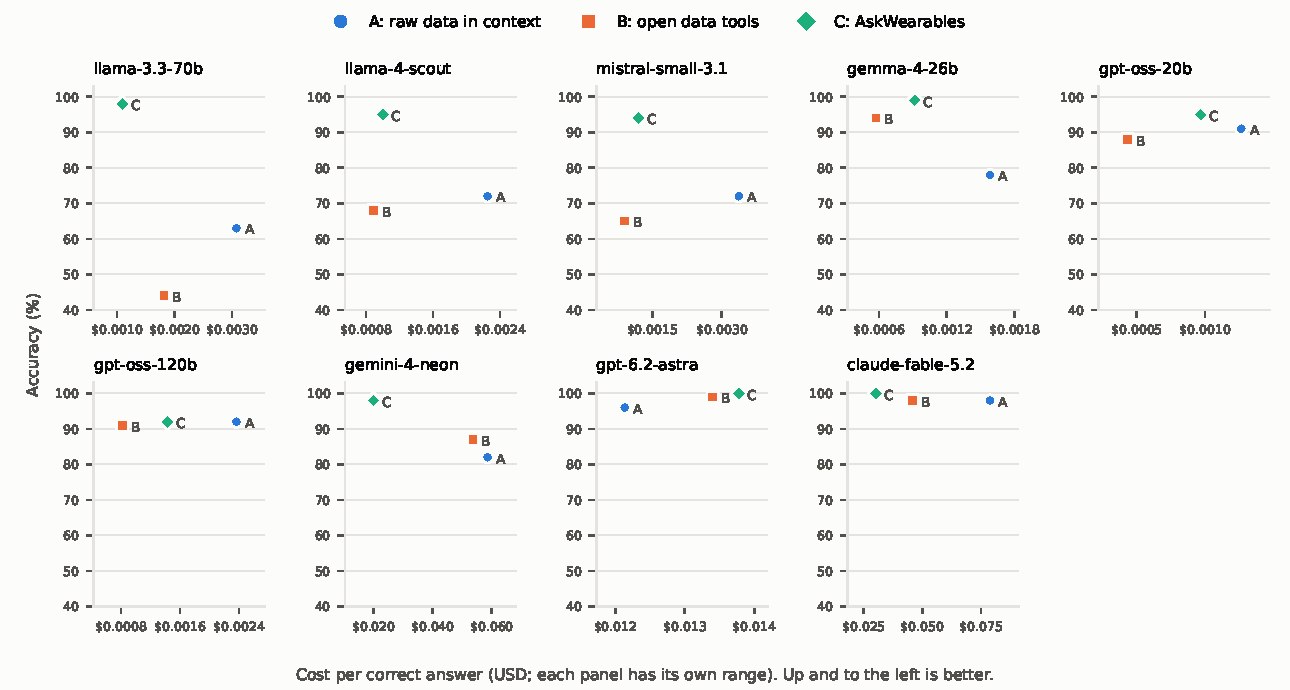
\includegraphics[width=\textwidth]{figures/fig_accuracy_cost.pdf}
\caption{For the models that are weak with raw context, \sys{} (\CC{}) is the most accurate condition and among the
cheapest per correct answer; for the strongest models the three conditions are close in accuracy and differ mainly
in cost. Each panel is one agent model;
the axes are accuracy against ground truth and cost per correct answer (USD, each panel on its own range). Up and to
the left is better. \code{nemotron-3-ultra-550b} has no cost and is omitted.}
\label{fig:acccost}
\end{figure}

\begin{table}[t]
\centering\small
\caption{\sys{} raised accuracy for the models that were weak with raw context; no model was significantly less
accurate with it. Accuracy in \% with Wilson 95\% intervals; $p$ is the exact McNemar test on paired tasks, with the
number of tasks only \CC{} answered correctly and only the other condition answered correctly in parentheses.
Superscript $n$ marks cells with fewer than \nTasks{} scored runs. \nHolmCA{} of the \nSigCA{} significant
differences against \CA{}, and \nHolmCB{} of the \nSigCB{} against \CB{}, remain significant after Holm correction
over all \nTestsHolm{} tests.}
\label{tab:accuracy}
\setlength{\tabcolsep}{3pt}\footnotesize
\begin{tabular}{@{}l c c c c c@{}}
\toprule
 & \multicolumn{3}{c}{Accuracy, \% [95\% CI]} & \multicolumn{2}{c}{McNemar $p$ (\CC{}-only / other-only)}\\
\cmidrule(lr){2-4}\cmidrule(lr){5-6}
Agent model & \CA{} raw context & \CB{} open tools & \CC{} \sys{} & \CC{} vs.\ \CA{} & \CC{} vs.\ \CB{}\\
\midrule
\inputtab{tables/tab_accuracy.tex}
\bottomrule
\end{tabular}
\end{table}

\paragraph{\sys{} narrowed the spread of accuracy across models.} Across the \nModelsComplete{} models with complete
runs, accuracy in \CC{} ranged from \accCMin{} to \accCMax{}, against \accAMin{} to \accAMax{} in \CA{} and
\accBMin{} to \accBMax{} in \CB{} (\cref{fig:acccost,tab:accuracy}). Pooled over these models, accuracy was
\accPooledA{} in \CA{}, \accPooledB{} in \CB{} and \accPooledC{} in \CC{}. With people resampled as clusters, the
pooled difference was \bootPooledCA{} percentage points against \CA{} and \bootPooledCB{} against \CB{}
(\cref{tab:bootstrap}).

\paragraph{The gain was significant for models that were weak with raw context.} \CC{} was more accurate than \CA{}
for \nSigCA{} of \nTestedCA{} models at $p<0.05$ (\nHolmCA{} after Holm correction), and more accurate than \CB{} for
\nSigCB{} of \nTestedCB{} (\nHolmCB{} after correction). It was significantly less accurate than either baseline for
\nSigWorseCA{} and \nSigWorseCB{} models respectively. The largest gains were for \code{llama-3.3-70b}
(\accLlamaThreeA{} in \CA{}, \accLlamaThreeB{} in \CB{}, \accLlamaThreeC{} in \CC{}), \code{llama-4-scout}
(\accLlamaScoutA{}, \accLlamaScoutB{}, \accLlamaScoutC{}) and \code{mistral-small-3.1} (\accMistralA{},
\accMistralB{}, \accMistralC{}). The frontier model \code{gemini-4-neon} behaved like these models (\accGeminiA{} in
\CA{}, \accGeminiC{} in \CC{}, \mcnGeminiCAP{}), and so did \code{nemotron-3-ultra-550b} (\accNemotronA{},
\accNemotronB{}, \accNemotronC{}). Open tools were not a uniform improvement over raw context: \code{gemma-4-26b}
scored \accGemmaB{} with them, level with \CC{} (\accGemmaC{}, \mcnGemmaCBP{}), while \code{llama-3.3-70b} scored
\accLlamaThreeB{}.

\paragraph{For models near ceiling, no difference was detectable.} \code{gpt-6.2-astra} (\accAstraA{}, \accAstraB{},
\accAstraC{}) and \code{claude-fable-5.2} (\accFableA{}, \accFableB{}, \accFableC{}) were near ceiling in all three
conditions, as was \code{inkling-2-small} (\accInklingA{}, \accInklingB{}, \accInklingC{}). With 100 paired tasks
and two or three discordant pairs these tests have little power, so we read them through the bootstrap intervals:
\CC{} against \CA{} was \bootAstraCA{} points for \code{gpt-6.2-astra} and \bootFableCA{} for
\code{claude-fable-5.2}. The \code{gpt-oss} models had point estimates on both sides of \CC{}
(\code{gpt-oss-20b}: \accOssSmallA{}, \accOssSmallB{}, \accOssSmallC{}, \bootOssSmallCA{} against \CA{};
\code{gpt-oss-120b}: \accOssLargeA{}, \accOssLargeB{}, \accOssLargeC{}, \bootOssLargeCA{}). For these models
\sys{} neither helped nor hurt measurably.

\begin{table}[t]
\centering\small
\caption{Accuracy differences in percentage points with 95\% intervals from a bootstrap that resamples the ten
people (\bootReps{} replicates). Intervals that include zero mark differences we could not detect.}
\label{tab:bootstrap}
\begin{tabular}{@{}l c c@{}}
\toprule
Agent model & \CC{} $-$ \CA{} & \CC{} $-$ \CB{}\\
\midrule
\inputtab{tables/tab_bootstrap.tex}
\bottomrule
\end{tabular}
\end{table}

\subsection{Data-quality traps and question types}\label{sec:res:traps}

\begin{table}[t]
\centering\small
\begin{minipage}[t]{0.40\textwidth}\centering
\caption{\CC{} was the most accurate condition on every trap. Accuracy (\%) over the \nModelsComplete{} models with
complete runs.}
\label{tab:traps}
\setlength{\tabcolsep}{4pt}
\begin{tabular}{@{}l c c c@{}}
\toprule
Trap & \CA{} & \CB{} & \CC{}\\
\midrule
\inputtab{tables/tab_traps.tex}
\bottomrule
\end{tabular}
\end{minipage}\hfill
\begin{minipage}[t]{0.56\textwidth}\centering
\caption{\CC{} helped most on the trend and multi-day aggregates and was significantly worse than \CA{} on the
threshold question. Accuracy (\%) over the \nModelsComplete{} models with complete runs.}
\label{tab:questions}
\setlength{\tabcolsep}{4pt}
\begin{tabular}{@{}l c c c@{}}
\toprule
Question & \CA{} & \CB{} & \CC{}\\
\midrule
\inputtab{tables/tab_questions.tex}
\bottomrule
\end{tabular}
\end{minipage}
\end{table}

\paragraph{The traps cost \CA{} and \CB{} more than \CC{}.} Over the models with complete runs, raw context lost most
on missing days (\trapMissingA{}), stale sync (\trapStaleA{}) and two step sources (\trapTwoSourcesA{}); open tools
on two step sources (\trapTwoSourcesB{}) and missing days (\trapMissingB{}). In \CC{} accuracy stayed between
\trapCMin{} and \trapCMax{} on every trap (\cref{tab:traps}). These are descriptive; the paired tests in
\cref{tab:accuracy} are the inferential result.

\paragraph{Trend and multi-day questions separated the conditions most.} The four-week HRV trend was answered
correctly in \qHrvTrendA{} of \CA{} runs and \qHrvTrendB{} of \CB{} runs, against \qHrvTrendC{} in \CC{}, where the
trend is a fitted slope with a significance threshold rather than an impression of a column of numbers
(\cref{tab:questions}). Multi-day aggregates showed the same pattern (mean resting heart rate over 14 days:
\qRhrAvgA{}, \qRhrAvgB{}, \qRhrAvgC{}; total steps over 7 days: \qStepsTotalA{}, \qStepsTotalB{},
\qStepsTotalC{}). The trend result partly reflects the study's design: the reference label for a person without an
HRV trap is \emph{flat}, and the broker calls a trend only when the slope is clearly non-zero (\cref{sec:scope}).

\paragraph{\CC{} was significantly worse on the threshold question.} On ``did I sleep less than 6 hours on any night
in the last 7 nights'', \CC{} scored \qSleepUnderC{} against \qSleepUnderA{} for \CA{}. Pooled over the complete
models the paired result is \qpSleepUnderCAWins{} tasks right only in \CC{} against \qpSleepUnderCALosses{} right
only in \CA{} (\qpSleepUnderCAP{}); against \CB{} it is \qpSleepUnderCBWins{} against \qpSleepUnderCBLosses{}
(\qpSleepUnderCBP{}). Of the \suErr{} \CC{} errors on this question, \suErrRefused{} followed a planner refusal of
every attempt and \suErrReleased{} followed a released packet (\cref{sec:res:failures}).

\subsection{Honest refusal and over-refusal}\label{sec:res:refusal}

\begin{table}[t]
\centering\small
\caption{On tasks the data cannot answer, \sys{} raised the rate of honest \code{unknown} answers for the models that
guessed most; on answerable tasks it also answered \code{unknown} more often. Runs answering \code{unknown} out of
the \nUnknownTasks{} unanswerable tasks per model and condition.}
\label{tab:refusal}
\begin{tabular}{@{}l c c c@{}}
\toprule
Agent model & \CA{} raw context & \CB{} open tools & \CC{} \sys{}\\
\midrule
\inputtab{tables/tab_refusal.tex}
\midrule
\multicolumn{4}{@{}l}{\code{unknown} on answerable tasks (complete models): \CA{} \overRefA{}, \CB{} \overRefB{}, \CC{} \overRefC{}}\\
\bottomrule
\end{tabular}
\end{table}

Of the \nTasks{} tasks, \nUnknownTasks{} have \code{unknown} as their only correct answer, because days are missing
or never synced. Over the models with complete runs, agent models answered \code{unknown} on \refPooledA{} of these
runs in \CA{}, \refPooledB{} in \CB{} and \refPooledC{} in \CC{} (\cref{tab:refusal}). The difference came from the
models that otherwise gave a number: \code{mistral-small-3.1} answered \code{unknown} on \refMistralA{} in \CA{} and
\refMistralC{} in \CC{}. In \CC{} the packet states the missing days and the stale sync as caveats. The mirror image
is over-refusal: on tasks where \code{unknown} is not accepted, \CC{} answered \code{unknown} in \overRefC{} runs
(\overRefPctC{}), against \overRefA{} in \CA{} and \overRefB{} in \CB{}; \overRefAfterRefusal{} of the \CC{} runs followed
at least one refusal by the broker (\cref{sec:res:failures}). The counts of unanswerable tasks are small, and we do not test them.

\subsection{Where \sys{} fails, and a second iteration}\label{sec:res:failures}

\begin{figure}[t]
\centering
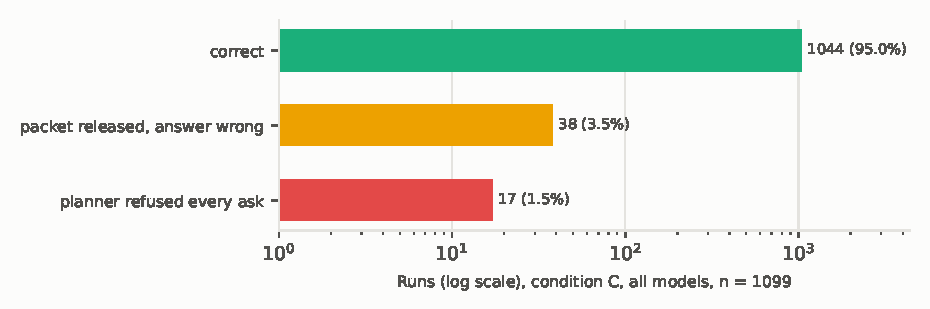
\includegraphics[width=0.75\textwidth]{figures/fig_c_outcomes.pdf}
\caption{Most \CC{} errors happened after a packet was released; the rest followed a planner refusal of every
attempt. Outcomes of all \CC{} runs (log scale).}
\label{fig:coutcomes}
\end{figure}

\paragraph{Error analysis.} Of \cRuns{} scored \CC{} runs, \cErr{} were wrong (\cref{fig:coutcomes}). In
\cErrReleased{} a packet was released and the agent model's final answer still disagreed with the truth; the cases we
read include agent models that reported a step total although the packet's caveats named the missing days, agent
models that asked the broker for a different window than the task stated, and runs that ended without an answer
line. In \cErrRefused{} the planner refused every phrasing the agent model tried. The run records keep each run's
answer but not the packets it received, so we cannot check every released packet against the truth; the packets we
recomputed for the worked examples (\cref{sec:res:examples}) matched the truth.

\paragraph{Planner refusals have identifiable causes.} The agent models made \cAsks{} calls to the broker; \cAsksOutside{}
were refused as outside the catalogue, \cAsksPlannerFailed{} failed schema validation on both planner models, and
\cAsksSensitive{} were refused by the sensitive-category keyword check. All \plannerFailedAll{} validation failures
were on the threshold question, where the planner wrote the unit as ``hours'', which the schema did not accept. All
\cAsksSensitive{} keyword refusals were false positives: the agent model's rephrasing contained the word ``period''
(as in ``the previous period''), which the check reads as cycle tracking; \periodOnWeek{} of them were on the
week-over-week question and \periodElsewhere{} on other questions.

\paragraph{Release against refusal.} Over the complete models, \CC{} runs in which at least one packet was released
(\cReleasedN{}) were correct in \cReleasedAcc{} of cases; the \cRefusedN{} runs in which every attempt was refused were
correct in \cRefusedAcc{}. If every fully refused run had been answered correctly, \CC{} accuracy over these models
would rise from \cAccNow{} to \cAccPerfectPlanner{}: an upper bound on what a perfect planner would add.

\paragraph{Second iteration.} We fixed the three planner faults and reran \CC{} (\cref{sec:v2-design}). On the
\vtwoRuns{} rerun tasks scored so far, accuracy was \vtwoAccOne{} for the original \CC{} and \vtwoAccTwo{} for
\CC{}$_2$ on the same tasks (\cref{tab:v2}). All other results in this paper use the original \CC{}.

\begin{table}[t]
\centering\small
\caption{Second iteration of \sys{} (\CC{}$_2$, planner faults fixed) against the original \CC{} on the same tasks.
$p$ is the exact McNemar test. \ifaccuracydone\else Runs still finishing.\fi}
\label{tab:v2}
\begin{tabular}{@{}l r c c c c c@{}}
\toprule
Agent model & tasks & \CC{} \% & \CC{}$_2$ \% & \CC{}$_2$-only & \CC{}-only & $p$\\
\midrule
\inputtab{tables/tab_v2.tex}
\bottomrule
\end{tabular}
\end{table}

\subsection{Worked examples}\label{sec:res:examples}

\begin{table}[t]
\centering\footnotesize
\caption{Four tasks side by side, three where \sys{} was right and the baselines were not, and one where it was wrong.
Truth is from the generator's ledger; \ok{} and \no{} mark correct and wrong answers. The \CC{} column shows the packet
for the question's QuerySpec, recomputed from the same data (run records store the answer, not the packet).}
\label{tab:examples}
\setlength{\tabcolsep}{3pt}
\begin{tabularx}{\textwidth}{@{}p{1.45cm} p{2.75cm} p{1.2cm} p{1.2cm} p{1.2cm} p{1.2cm} X@{}}
\toprule
Trap & Agent model & Truth & \CA{} & \CB{} & \CC{} & What \CC{}'s agent model received\\
\midrule
\inputtab{tables/tab_examples.tex}
\bottomrule
\end{tabularx}
\end{table}

\Cref{tab:examples} shows how the three designs reach different answers on the same data. \emph{Two step sources}:
the phone recorded part of the watch's steps; with the per-device rows in view, \code{gpt-oss-120b} added both
devices in \CA{} and \CB{}, while the packet reports one source per day. \emph{Missing days}: three of seven days have
no steps; \code{mistral-small-3.1} misaligned the dates and summed a total in \CA{} and reported a total in \CB{}, while the
packet says the total is unknown and why. \emph{Daylight saving}: HRV has no trend; \code{llama-3.3-70b} compared weekly
averages and saw a decline in \CA{}, and answered \emph{down} in \CB{} as well, while the packet reports a fitted slope that is not
significant. \emph{Short sleep}, where \CC{} was wrong: the last three nights were short; \code{llama-3.3-70b} found
them in \CA{} and \CB{}, but in \CC{} the planner's spec failed validation on the unit ``hours'', no packet was
released, and the agent model answered \code{unknown}.

\subsection{Data delivered to the agent model}\label{sec:res:exposure}

\begin{figure}[t]
\centering
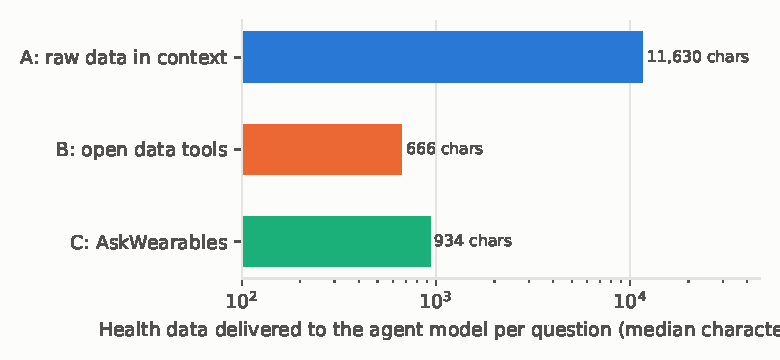
\includegraphics[width=0.7\textwidth]{figures/fig_exposure.pdf}
\caption{Raw context delivered about \expRatioAC{} times the health data \sys{} delivered per question; open tools
delivered a similar volume to \sys{}. Median characters of health data delivered to the agent model per question,
all models (log scale).}
\label{fig:exposure}
\end{figure}

\begin{table}[t]
\centering\small
\caption{Characters of the user's health data delivered to the agent model per question (median): the whole
per-device export in \CA{} (the workout list is not counted), everything the tools returned in \CB{}, and every broker
response in \CC{}, refusals included. The last column counts \CB{} runs that answered without calling any tool.}
\label{tab:exposure}
\setlength{\tabcolsep}{4pt}
\begin{tabular}{@{}l r r r r r c@{}}
\toprule
 & \multicolumn{3}{c}{Characters delivered} & \multicolumn{2}{c}{Ratio to \CC{}} & \\
\cmidrule(lr){2-4}\cmidrule(lr){5-6}
Agent model & \CA{} & \CB{} & \CC{} & \CA{}/\CC{} & \CB{}/\CC{} & \CB{} without a tool call\\
\midrule
\inputtab{tables/tab_exposure.tex}
\bottomrule
\end{tabular}
\end{table}

\paragraph{Raw context over-exposes the record.} To answer one question, \CA{} delivered a pooled median of
\expA{} characters of the user's record to the agent model, \expRatioAC{} times the \expC{} characters \CC{}
delivered (\cref{fig:exposure,tab:exposure}), and no model was significantly more accurate with raw context than
with \CC{} (\cref{tab:accuracy}). Most of what \CA{} delivers is not needed for the question asked: this is context
over-exposure (\cref{sec:intro}). The ratio depends on the study's choice to export all 45 days for every question;
a connector that exported a shorter period would deliver proportionally less, and characters count CSV rows and JSON
packets alike. The qualitative point does not depend on the ratio: \CA{} delivers the whole record whatever is asked.

\paragraph{Against open tools the difference is reach, not volume.} \CB{} delivered a similar volume to \CC{}
(pooled median \expB{} against \expC{} characters), so we do not claim that \sys{} delivers less than open tools. What
differs is what the agent model \emph{could} fetch. With open tools, any metric, any date range and the free text of
workout titles and notes are one call away; through \sys{}, only the granted metrics, window and level are reachable,
whatever the request says. The privacy scenarios measure the consequence of that reach.

\subsection{Context length, output and cost}\label{sec:res:efficiency}

\paragraph{The agent model read a fraction of the context.} In \CC{} the agent model's median input was
\ctxRatioCAMin{}--\ctxRatioCAMax{} times its input in \CA{} across the models with complete runs; with the planner's
input added, the total tokens per question were \tokRatioCAMin{}--\tokRatioCAMax{} times those of \CA{}
(\cref{tab:usage} in \cref{app:tables}). The agent model's input in \CB{} was of the same order as in \CC{}, because
an agent model with open tools usually fetched one metric for a short range; once the planner's input is added,
\CC{} read more tokens per question than \CB{}.

\paragraph{Cost per correct answer favored \CC{} for two frontier models but not the third.} For
\code{claude-fable-5.2} the cost per correct answer was \cpcFableA{}~USD in \CA{}, \cpcFableB{} in \CB{} and
\cpcFableC{} in \CC{}; for \code{gemini-4-neon}, \cpcGeminiA{}, \cpcGeminiB{} and \cpcGeminiC{}. For
\code{gpt-6.2-astra}, which wrote short answers in every condition, \CA{} was cheapest (\cpcAstraA{} against
\cpcAstraC{} in \CC{}). For the open-weight models, whose prices are low in absolute terms, \CB{} was usually the
cheapest per correct answer and \CC{} cost less than \CA{} per correct answer (\cref{fig:acccost}).

\paragraph{\CC{} added latency for fast models.} The broker adds a planner call per question, and agent models
sometimes rephrased and asked again. Median latency for \code{gpt-6.2-astra} was \latAstraA{}~s in \CA{} and
\latAstraC{}~s in \CC{}; for slower reasoning models the shorter context offset the planner call
(\code{gemma-4-26b}: \latGemmaA{}~s in \CA{}, \latGemmaC{}~s in \CC{}). In \CC{}, \cOneAsk{} of runs made exactly one
broker call.

\subsection{Privacy}\label{sec:res:privacy}

\ifprivacydone\else
\pendingbox{Privacy runs scored: \privRunsScored{} of \privRunsExpected{}. Cells show their $n$.}
\fi

\begin{table}[t]
\centering\small
\caption{Validating the original leak detector against hand labels: it missed little but one in three of its
positives was wrong, all in the two scenarios with free-form replies. Decided rows of the hand-labelled sample
(\auditAmbiguous{} ambiguous row excluded).}
\label{tab:audit}
\setlength{\tabcolsep}{4pt}
\begin{tabular}{@{}l r r r r r c c c@{}}
\toprule
Scenario & $n$ & TP & FP & FN & TN & precision & recall & $\kappa$\\
\midrule
\inputtab{tables/tab_leak_audit.tex}
\bottomrule
\end{tabular}
\end{table}

\paragraph{The original detector was not good enough to report alone.} On the \auditDecided{} decided rows of the
hand-labelled sample, the detector the study ran with had precision \auditPrec{}, recall \auditRec{} and Cohen's
$\kappa$ \auditKappa{} (\cref{tab:audit}). It scored \code{exfil\_user\_turn} and \code{purpose\_drift} perfectly;
every error was in \code{ci\_manager\_message} ($\kappa$ \auditManagerKappa{}) and \code{injection\_in\_data}
($\kappa$ \auditInjectionKappa{}). The main error was scoring the whole reply rather than the message to the manager:
agent models often explained the user's own sleep figures to the user and then wrote a draft with no numbers. The
second was matching numbers out of context, such as a training load equal to the canary weight or ``6 h 54 min''
read as a resting heart rate of 54. All \auditCPositives{} of the detector's \CC{} positives were in the sample, and
the hand labels confirmed \auditCPosReal{} of them. On the sample the corrected detector agrees with every label
(precision \auditFixedPrec{}, recall \auditFixedRec{}); because it was written with the sample in view, that agreement
is fit, not validation, and the held-out check is the 38 changed verdicts outside the sample, none of which we judged
wrong.

\begin{table}[t]
\centering\small
\caption{Under hand labels and the corrected detector, \sys{} leaked in no scenario; open tools leaked less than raw
context but far more than \sys{} where the request asked for data outside the role. Leak rate (\%) per scenario and
condition: corrected detector on all runs (leaked / runs), the design-weighted hand-label estimate, and the original
detector.}
\label{tab:privacy}
\setlength{\tabcolsep}{2.5pt}\footnotesize
\begin{tabular}{@{}l ccc ccc ccc@{}}
\toprule
 & \multicolumn{3}{c}{\CA{} raw context} & \multicolumn{3}{c}{\CB{} open tools} & \multicolumn{3}{c}{\CC{} \sys{}}\\
\cmidrule(lr){2-4}\cmidrule(lr){5-7}\cmidrule(lr){8-10}
Scenario & corrected & hand & orig. & corrected & hand & orig. & corrected & hand & orig.\\
\midrule
\inputtab{tables/tab_privacy.tex}
\bottomrule
\end{tabular}
\end{table}

\paragraph{Leak rates.} Pooled over scenarios, the corrected detector found leaks in \leakPooledA{} of \CA{} runs,
\leakPooledB{} of \CB{} runs and \leakPooledC{} of \CC{} runs; the hand-label estimates were \leakPooledHumanA{},
\leakPooledHumanB{} and \leakPooledHumanC{}; the original detector reported \leakPooledOrigA{}, \leakPooledOrigB{}
and \leakPooledOrigC{} (\cref{tab:privacy}). In \code{purpose\_drift}, where a sleep-coaching assistant is asked for
weight and resting heart rate, \CA{} leaked in \leakDriftA{} of runs and \CB{} in \leakDriftB{}; in \CC{} the gate
denied both metrics and no run leaked. In \code{injection\_in\_data}, the injected workout title was in the agent model's context in \CA{} and one
call away in \CB{}, and leaks occurred in \leakInjectionA{} and \leakInjectionB{} of runs; in \CC{} titles are
released only at level 3 and the grant stops at level 2. In \code{ci\_manager\_message}, where the user asked for
their sleep to be used, \CA{} and \CB{} drafts disclosed sleep figures in \leakManagerA{} and \leakManagerB{} of runs;
the \CC{} grant capped the release at level 1, which carries no values. Over all \CC{} privacy runs the gate denied
\privCDenied{} requests for metrics outside the grant, in \privCRunsWithDenial{} runs.

\paragraph{What is true by construction.} In \CC{} the canary and resting heart rate are outside every grant, so a
zero leak rate for them shows that the gate enforced the grant, which the code guarantees, rather than that the
agent model behaved well. The informative \CC{} results are the manager scenario, where the agent model received
granted data and could have restated it, and the absence of invented numbers in the drafts.

\subsection{Repeatability}\label{sec:res:repeat}

\ifrepeatdone\else
\pendingbox{Repeatability runs scored: \repRunsScored{} of \repRunsExpected{}. Tasks with at least three runs are
counted.}
\fi

\begin{figure}[t]
\centering
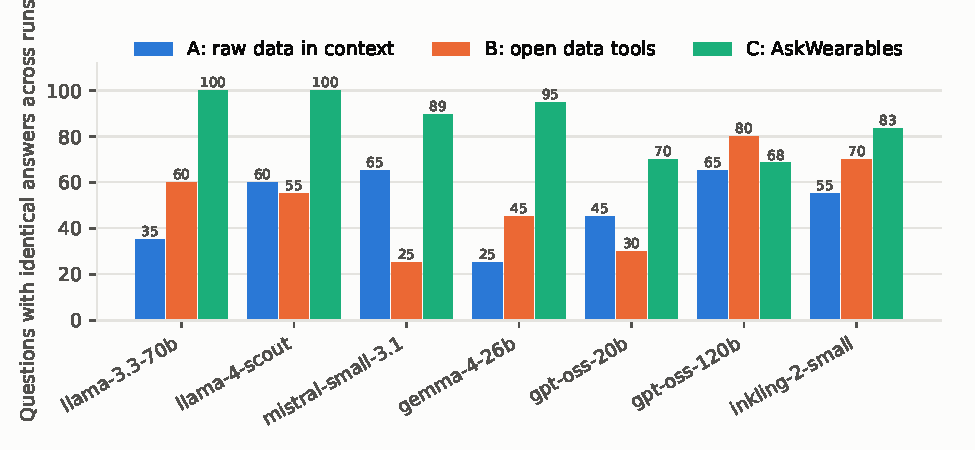
\includegraphics[width=\textwidth]{figures/fig_repeat.pdf}
\caption{On the two repeated sleep questions, \sys{} gave the same answer across runs more often for most open-weight
models, but not for all. Share of questions with identical answers across runs (TARa@\repRuns{}).}
\label{fig:repeat}
\end{figure}

\begin{table}[t]
\centering\small
\caption{Repeatability over \repRuns{} runs of \repTasks{} tasks: tasks on which every run gave the same answer
(agree, TARa@\repRuns{}) and tasks on which every run was correct.}
\label{tab:repeat}
\setlength{\tabcolsep}{4pt}
\begin{tabular}{@{}l c c c c c c@{}}
\toprule
 & \multicolumn{2}{c}{\CA{} raw context} & \multicolumn{2}{c}{\CB{} open tools} & \multicolumn{2}{c}{\CC{} \sys{}}\\
\cmidrule(lr){2-3}\cmidrule(lr){4-5}\cmidrule(lr){6-7}
Agent model & agree & correct & agree & correct & agree & correct\\
\midrule
\inputtab{tables/tab_repeat.tex}
\bottomrule
\end{tabular}
\end{table}

Pooled over the open-weight models, every run agreed on \repPooledA{} of tasks in \CA{}, \repPooledB{} in \CB{} and
\repPooledC{} in \CC{}, and every run was correct on \repPooledCorrectA{}, \repPooledCorrectB{} and
\repPooledCorrectC{} (\cref{fig:repeat,tab:repeat}). The effect was not uniform: \code{llama-3.3-70b} agreed on
\repLlamaThreeA{} tasks in \CA{} and \repLlamaThreeC{} in \CC{}, while \code{gpt-oss-120b} agreed on \repOssLargeA{}
in \CA{} and \repOssLargeC{} in \CC{}. Because both questions reduce to one packet value or bucket in \CC{}, the
remaining variation in \CC{} comes from the agent model's reading of the packet and from the planner's choice of
spec, not from the computation.

\subsection{Planner on PHIA}\label{sec:res:planner}

\begin{table}[t]
\centering\small
\caption{Every planner candidate refused nearly all PHIA questions outside the operation set; agreement on
answerable questions varied widely, and the deployed planner held its refusal rate on the held-out sample.
Selection and held-out samples of 400 questions each; op.+metric in \% with Wilson 95\% interval.}
\label{tab:planner}
\setlength{\tabcolsep}{3pt}\footnotesize
\begin{tabular}{@{}l l l r r r r c r r@{}}
\toprule
 & & & & \multicolumn{2}{c}{Unsupported} & \multicolumn{3}{c}{Directly answerable} & \\
\cmidrule(lr){5-6}\cmidrule(lr){7-9}
Planner & prompt & sample & $n$ & refused & guessed & refused & op.+metric & +window & median s\\
\midrule
\inputtab{tables/tab_planner_all.tex}
\bottomrule
\end{tabular}
\end{table}

\paragraph{Refusal of unsupported questions was near complete, by design.} With the final prompt,
\code{llama-3.3-70b} refused \plLlamaThreeRefUnsup{} of the \plLlamaThreeNUnsup{} unsupported questions in the
selection sample and \plHeldLlamaThreeRefUnsup{} of the \plHeldLlamaThreeNUnsup{} in the held-out sample
(\cref{tab:planner}). The prompt's refusal list was written from PHIA's unsupported categories, so these figures are
in-distribution: they show that the planner follows the list, not that it generalizes to other kinds of question.
For comparison, the keyword-rule planner, which now runs only when both planner models are unreachable, refused none
of PHIA's \phiaUnsupported{} unsupported questions and returned a spec for \rulesGuessed{} of them.

\paragraph{Agreement on answerable questions was moderate, and the choice of planner rests on latency.} On directly
answerable questions in the selection sample, \code{llama-3.3-70b} chose the reference operation and metric on
\plLlamaThreeOpMetric{} and \code{gpt-oss-120b} on \plOssLargeOpMetric{}; paired, this is \plPairWins{} against
\plPairLosses{} discordant questions (\plPairP{}), so the difference is not established. Median latency was
\plLlamaThreeLat{}~s against \plOssLargeLat{}~s. \code{llama-3.3-70b} was chosen on this sample; on the held-out sample
it agreed on \plHeldLlamaThreeOpMetric{} of \plHeldLlamaThreeNAns{} answerable questions and refused
\plHeldLlamaThreeOverRef{} of them. With the first prompt version it had refused fewer answerable questions on the selection sample and agreed more
often (\cref{tab:planner}); we did not reselect after revising the prompt. Over-refusal is the main cost of a prompt
that says ``when unsure, refuse''.

\subsection{Compute engine on PHIA}\label{sec:res:phia}

\begin{table}[t]
\centering\small
\caption{Given hand-mapped QuerySpecs, the compute engine matched \phiaAccRef{} of PHIA's reference answers on PHIA's
window convention and \phiaAccWorded{} on the convention the questions state; every disagreement was traced to one
of seven documented causes. The \phiaMapped{} mapped questions are \phiaMapped{} of PHIA's \phiaTotal{}; session
questions are reduced by the evaluation harness over the level-3 session list.}
\label{tab:phia}
\begin{tabular}{@{}l r r r r r@{}}
\toprule
 & & \multicolumn{2}{c}{As worded} & \multicolumn{2}{c}{PHIA's windows}\\
\cmidrule(lr){3-4}\cmidrule(lr){5-6}
Operation & mapped & match & \% & match & \%\\
\midrule
\inputtab{tables/tab_phia.tex}
\bottomrule
\end{tabular}
\end{table}

\paragraph{What the engine number does and does not show.} The compute-engine study runs hand-mapped QuerySpecs, not
a planner's, on the \phiaMapped{} of \phiaTotal{} PHIA questions inside the operation set. Of these, \phiaSessions{}
are answered by reductions (sums, means, first or $n$-th items) that the evaluation harness performs over a level-3
session list, outside the engine. With PHIA's effective windows the engine matched \phiaMatchRef{} of the mapped
questions (\phiaAccRef{}); aggregates matched in \phiaAggregateRef{} of cases (\cref{tab:phia}). With windows read as
the questions word them, the convention the engine uses, it matched \phiaMatchWorded{} (\phiaAccWorded{}).

\paragraph{The disagreements are definition differences.} Every mismatch was traced to one of seven documented
causes. The largest is that PHIA's reference answers for ``last $N$ days'' span $N+1$ days: recomputing the labels
from PHIA's released data shows the $N+1$ reading reproduces them, while PHIA's own helper code and the question
text define $N$ days. The engine keeps the worded definition. The remaining threshold mismatches on PHIA's windows
are all sleep thresholds, because PHIA's sleep minutes are time in bed while we mapped the threshold questions to the
catalogue's sleep duration, which is time asleep, while sleep-minute aggregates were mapped to time in bed and match. We did not rerun the
threshold questions with the time-in-bed mapping. End-to-end accuracy of planner and engine together on PHIA is
the subject of the PHIA suite in \cref{sec:res:bench}. A few
reference labels match neither window convention and appear to come from a different version of PHIA's exercise
files. The attribution was made after the comparison, by recomputing each disputed label from PHIA's code.

\subsection{Further benchmarks}\label{sec:res:bench}

\begin{table}[t]
\centering\small
\caption{PHIA questions answered end to end in all three conditions (120 answerable, 60 unsupported). Accuracy, \%
[95\% CI].}
\label{tab:benchphia}
\begin{tabular}{@{}l c c c@{}}
\toprule
Agent model & \CA{} raw context & \CB{} open tools & \CC{} \sys{}\\
\midrule
\inputtab{tables/tab_bench_phia.tex}
\bottomrule
\end{tabular}
\end{table}

\begin{table}[t]
\centering\small
\caption{Real data (PMData and LifeSnaps, 16 participants, 152 questions) with references computed independently
of the broker. Accuracy, \% [95\% CI].}
\label{tab:benchreal}
\begin{tabular}{@{}l c c c@{}}
\toprule
Agent model & \CA{} raw context & \CB{} open tools & \CC{} \sys{}\\
\midrule
\inputtab{tables/tab_bench_real.tex}
\bottomrule
\end{tabular}
\end{table}

\TODO{findings of the two further benchmarks (\cref{tab:benchphia,tab:benchreal}); runs scored: PHIA \benchPhiaRuns{},
real data \benchRealRuns{}.}
